
\subsection{Heuristics --- issues, comments and observations}

A complete and full list of usability issues found mapped to the appropriate heuristic with evaluator assigned severity level can be found in \S\ref{sect:heuristicresults}. Figure~\vref{fig:issues} shows the number of issues found per heuristic. This doesn't reflect the total number of issues found, as some issues are related to multiple heuristics.

\begin{figure}[!htb]
	\centering
	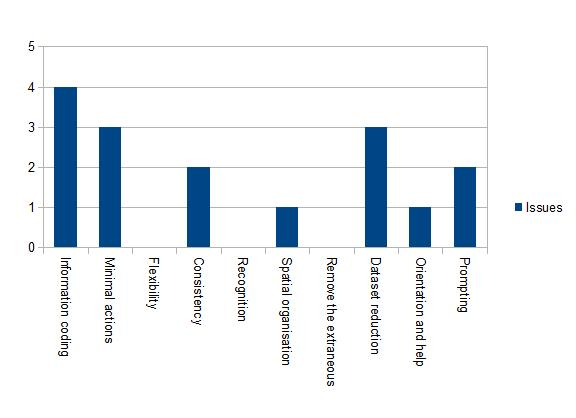
\includegraphics[scale=0.70]{issues.jpg}
	\caption{\textit{Number of issues per heuristic (issues may be related to more than one heuristic)}}
	\label{fig:issues}
\end{figure}

\paragraph{Initial presentation of dataset}
Evaluators thought that the initial starting point when exploring unknown data was confusing. Some users felt that it would be helpful to have the cloud pre-mapped to data fields and a starting cloud displayed on initiation of the software. The default mappings select all options except for transparency. Users felt that starting with just one mapping and adding others as needed was more useful to build knowledge about the dataset.

\paragraph{Selection of data mappings}
The mapping selections were perceived to be the major area which needed improvement. Although not given specific tasks, users quickly ascertained what useful questions might be asked of a dataset (e.g. what club has the best cross country runners?), but had some difficulty selecting mappings that might help them answer these questions. What was useful for decision making in mapping selection was an overview of each variable as a starting point for further investigation (e.g. what is the data range for this variable? Is it text or numerical? Is it categorical?). This information had been provided for them on paper (Table~\vref{table:datasetheuristiceval}), but users commented it would be useful information to integrate into the tool. As a result of initial misunderstandings over data field type, users were sometimes confused by mapping variables to textual data instead of numerical data (this is not useful for mapping to some visual properties such as font size). Conversely, evaluators didn't always map the text label to the tag text but used an numeric ID column. While not as immediately/obviously useful as mapping text, this did have the added advantages of maximising space efficiency in the visualisation, minimising the overemphasising effect of long text and allowing the user to gain an overview of the data in the ID column (ranges for example).

Users didn't use the transparency mapping much at all --- it wasn't perceived to be as useful as font size or colour, and some users were confused by the transparency mapping interface. The drop-down box for layout was confusing as it contained layout options that were for layout research purposes. Evaluators didn't change the default colour set much, although one user commented that black and white were the most helpful colour combinations. A suggestion was made for data to be more complemented by the colour legend. It would be useful for categorical data to be displayed as a colour for every category in a data field.

Another feature requested for mapping selection was the reversal of the mappings properties. This was available for the ordering property but not for size or colour. An evaluator noted that data wasn't always best displayed from smallest to largest numeric value.

\paragraph{Static and dynamic filtering}

Most time was spent by users changing mappings rather than filtering data. One user remarked that this was because of the free exploration nature of the evaluation --- if we had asked more specific questions about the dataset, then more time would have been spent filtering the data to a more appropriate subset according to the question.

The mouse wheel filter was a dynamic filter (appearing on static tab). It was suggested that it would be more useful as a static filter --- useful to discover what settings are most appropriate to display --- and should stay observed after the reset/update button click. This option is not known to the user until they select the filter tab. The dynamic filtering interface was problematic for one user as they didn't realise they could select the knobs on the slider.

\paragraph{Visual encoding}

The visualisation itself didn't pose too many problems for the users. One user wasn't aware of the overview right click pop-up because of an oversight in the training. A complaint about typewriter layout was that it created a disjoint in the flow of the data field mapped to order at the end of each row.

\subsection{Heuristics --- guideline checklist}

The guideline checklist can be found in \S\ref{sect:checklist}. Evaluators were asked to mark each guideline specifying whether they considered each criteria fulfilled, not fulfilled, or partially fulfilled. Each figure visualising results of a heuristic presents marks averaged from  evaluators on a scale between zero and one (where zero means the criteria is not fulfilled, and one means the criteria is fulfilled). This section summarises and discusses guideline checklist results for each heuristic.

\begin{figure}[!htb]
\centering
\begin{subfigure}{.5\textwidth}
	\centering
	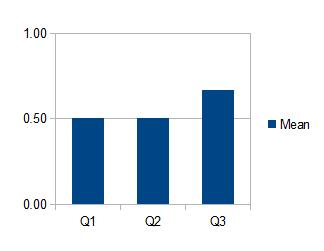
\includegraphics[scale=0.65]{informationcoding.jpg}
\end{subfigure}%
\begin{subfigure}{.5\textwidth}
  \begin{description}
	\item[Q1]Are the data to visual element mappings understandable and effective?
	\item[Q2]Is the use of additional symbols in the representation understandable and effective? 
	\item[Q3]Can you get a general understanding of the underlying data values of an individual item and where the individual data item fits into the overall dataset?
  \end{description}
\end{subfigure}
\caption{\textit{Information coding --- visual representation}}
\label{fig:informationcoding}
\end{figure}

\paragraph{Information coding --- visual representation (Figure~\vref{fig:informationcoding})}

Evaluators felt this criterion was partially fulfilled. One evaluator felt that an overall understanding of the underlying dataset was only possible after a user had some experience or practice with the system. We felt that the responses to this guideline reflected the problems evaluators found with the mapping selection interface. 

\begin{figure}[!htb]
\centering
\begin{subfigure}{.5\textwidth}
	\centering
	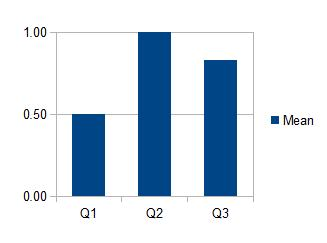
\includegraphics[scale=0.65]{minimalactions.jpg}
\end{subfigure}%
\begin{subfigure}{.5\textwidth}
  \begin{description}
	\item[Q1]Are the number of steps required to perform a task reasonable?
	\item[Q2]For data entry, are currently defined default values displayed in their appropriate data fields?
	\item[Q3]Can the user directly go to a requested view, without having to go through intermediaries?
  \end{description}
\end{subfigure}
\caption{\textit{Minimal actions --- interactivity}}
\label{fig:minactions}
\end{figure}

\paragraph{Minimal actions --- interactivity (Figure~\vref{fig:minactions})}

This criterion was generally satisfied. Issues regarding the number of steps required to perform a task were interpreted as relating to default mapping values and the initial display of the dataset. 

\begin{figure}[!htb]
\centering
\begin{subfigure}{\textwidth}
	\centering
	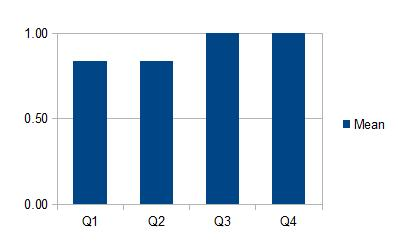
\includegraphics[scale=0.80]{flexibility.jpg}
\end{subfigure}
\begin{subfigure}{\textwidth}
  \begin{description}
	\item[Q1]Are users provided with sufficient means to control visualisation configuration?
	\item[Q2]Are users permitted to define, change or remove default values for settings?
	\item[Q3]When some displays are unnecessary, can users remove or hide them temporarily?
	\item[Q4]Can users change settings in any order?
  \end{description}
\end{subfigure}
\caption{\textit{Flexibility --- interactivity}}
\label{fig:flexibility}
\end{figure}

\paragraph{Flexibility --- interactivity (Figure~\vref{fig:flexibility})}

Evaluators were satisfied that the system provided sufficient flexibility in controlling tag cloud configuration.

\begin{figure}[!htb]
\centering
\begin{subfigure}{\textwidth}
	\centering
	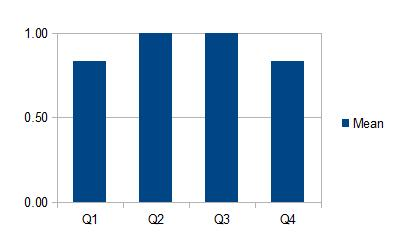
\includegraphics[scale=0.80]{consistency.jpg}
\end{subfigure}
\begin{subfigure}{\textwidth}
  \begin{description}
	\item[Q1]Are window titles always located in the same place?
	\item[Q2]Are the configuration controls consistent?
	\item[Q3]Are similar procedures used to perform tasks?
	\item[Q4]Are labels (phrasing, punctuation, placement) consistent?
  \end{description}
\end{subfigure}
\caption{\textit{Consistency --- interactivity}}
\label{fig:consistency}
\end{figure}

\paragraph{Consistency --- interactivity (Figure~\vref{fig:consistency})}

Criterion was satisfied for consistency in user interface --- configuration controls, window titles, labels and general task procedures. 

\begin{figure}[!htb]
\centering
\begin{subfigure}{.5\textwidth}
	\centering
	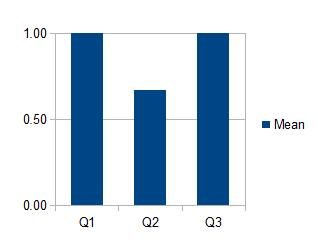
\includegraphics[scale=0.65]{recognition.jpg}
\end{subfigure}%
\begin{subfigure}{.5\textwidth}
  \begin{description}
	\item[Q1]Are the available user actions visible to the user?
	\item[Q2]Can the user perform tasks without having to recall information?
	\item[Q3]Can tasks be performed without referring to external documentation?
  \end{description}
\end{subfigure}
\caption{\textit{Recognition rather than recall --- interactivity}}
\label{fig:recognition}
\end{figure}

\paragraph{Recognition rather than recall --- interactivity (Figure~\vref{fig:recognition})}

This criterion was generally satisfied although evaluators wanted greater access to summary information relating to the dataset.

\begin{figure}[!htb]
\centering
\begin{subfigure}{\textwidth}
	\centering
	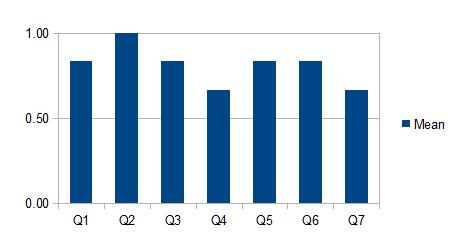
\includegraphics[scale=0.80]{organisation.jpg}
\end{subfigure}
\begin{subfigure}{\textwidth}
  \begin{description}
	\item[Q1]Can I easily locate an information element in the display?
	\item[Q2]Are the individual elements legible?
	\item[Q3]Is space used efficiently in the layout?
	\item[Q4]Am I aware of the overall distribution of information elements in the representation?
	\item[Q5]Are some objects occluded by others?
	\item[Q6]Does the layout follow a logical organisation?
	\item[Q7]Do I understand how tag placement is related to the selected layout and ordering? 
  \end{description}
\end{subfigure}
\caption{\textit{Spatial organisation --- visual representation}}
\label{fig:organisation}
\end{figure}

\paragraph{Spatial organisation --- visual representation (Figure~\vref{fig:organisation})}

Evaluators rated Taggle fairly well for this criteria. One comment regarding the spatial aspect of the visualisation was that the tag cloud could sometimes be very small in the middle of the canvas which wasn't an efficient use of space. This depended on the data mapped though. Another evaluator commented that layout may or may not follow a logical organisation because it depended on their own appropriate mapping selections.

\begin{figure}[!htb]
\centering
\begin{subfigure}{.5\textwidth}
	\centering
	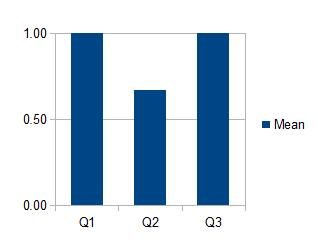
\includegraphics[scale=0.65]{extraneous.jpg}
\end{subfigure}%
\begin{subfigure}{.5\textwidth}
  \begin{description}
	\item[Q1]Are means provided to reduce the distracting effect of extra information when locating information?
	\item[Q2]Are means provided to reduce the distracting effect of extra information when gaining an overview?
	\item[Q3]Are means provided to reduce the distracting effect of extra information when making a comparison?
  \end{description}
\end{subfigure}
\caption{\textit{Remove the extraneous --- interactivity }}
\label{fig:extraneous}
\end{figure}

\paragraph{Remove the extraneous --- interactivity (Figure~\vref{fig:extraneous})}

This criteria was marked as partially met. Evaluators felt that it was important to get a simplified overview of the dataset initially which hadn't been provided for in the interface.

\begin{figure}[!htb]
\centering
\begin{subfigure}{.5\textwidth}
	\centering
	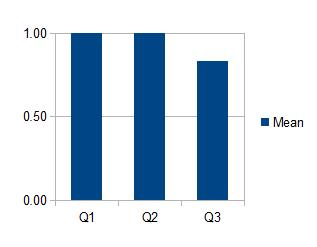
\includegraphics[scale=0.65]{reduction.jpg}
\end{subfigure}%
\begin{subfigure}{.5\textwidth}
  \begin{description}
	\item[Q1]Are means provided to filter/reduce a dataset?
	\item[Q2]Are means provided to ``prune'' or cut off information that may be irrelevant?
	\item[Q3]Are filtering mechanisms efficient and easy to use?
  \end{description}
\end{subfigure}
\caption{\textit{Dataset reduction --- interactivity }}
\label{fig:reduction}
\end{figure}

\paragraph{Dataset reduction --- interactivity (Figure~\vref{fig:reduction})}

Evaluators were satisfied that the system provided sufficient means for filtering and reducing the dataset.

\begin{figure}[!htb]
\centering
\begin{subfigure}{.5\textwidth}
	\centering
	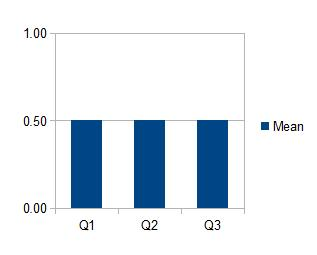
\includegraphics[scale=0.65]{help.jpg}
\end{subfigure}%
\begin{subfigure}{.5\textwidth}
  \begin{description}
	\item[Q1]Are means provided to control levels of detail?
	\item[Q2]Are means provided to redo/undo user actions?
	\item[Q3]Is requested additional information represented, or accessible?
  \end{description}
\end{subfigure}
\caption{\textit{Orientation and help --- interactivity }}
\label{fig:help}
\end{figure}

\paragraph{Orientation and help --- interactivity (Figure~\vref{fig:help})}

Evaluators felt help interactivity was only partially satisfied. More assistance could be provided to orientate the user to the system through means such as redo and undo. 

\begin{figure}[!htb]
\centering
\begin{subfigure}{\textwidth}
	\centering
	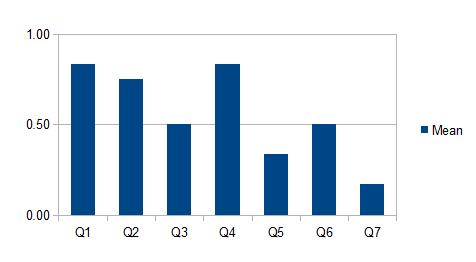
\includegraphics[scale=0.80]{prompting.jpg}
\end{subfigure}
\begin{subfigure}{\textwidth}
  \begin{description}
	\item[Q1]Are users aware of valid values for interface options?
	\item[Q2]Are measurement units displayed for data entry?
	\item[Q3]Is status information displayed?
	\item[Q4]Are labels provided for all fields?
	\item[Q5]Are cues provided on the acceptable length of data entries?
	\item[Q6]Are titles provided for each window?
	\item[Q7]Is online help and guidance provided?
  \end{description}
\end{subfigure}
\caption{\textit{Prompting --- interactivity}}
\label{fig:prompting}
\end{figure}

\paragraph{Prompting --- interactivity (Figure~\vref{fig:prompting})}

As with orientation and help, evaluators felt the prompting status of Taggle could be improved with the addition of things such as online help and more cues on acceptable data entries. We feel manuals and online help guides are more useful and expected for a mature tool rather than a prototype.


\subsection{Questionnaire}

This section presents results for a 5-point Likert scale questionnaire where evaluators were asked to rate the tool with regards to comprehensibility, knowledge discovery support, and other research questions from 1 (``Strongly disagree'') to 5 (``Strongly agree''). Results for each questionnaire section are summarised and discussed.

\begin{figure}[!htb]
\centering
\begin{subfigure}{\textwidth}
	\centering
	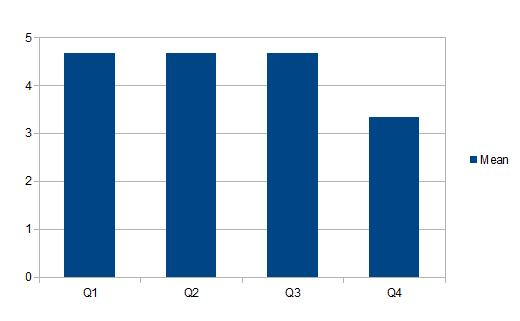
\includegraphics[scale=0.60]{comprehensible.jpg}
\end{subfigure}
\begin{subfigure}{\textwidth}
  \begin{description}
	\item[Q1]I immediately understood that underlying data values between large tags and small tags were different
	\item[Q2]I immediately understood that underlying data values between tags with contrasting colours were different
	\item[Q3]I immediately understood that underlying data values between tags with contrasting transparency levels were different
	\item[Q4]When looking at a visualisation the tag label gave me an immediate visual clue as to the kind of data the tag was representing
  \end{description}
\end{subfigure}
\caption{\textit{Is the visualisation technique instinctively comprehensible?}}
\label{fig:comprehension}
\end{figure}

\paragraph{Is the visualisation technique instinctively comprehensible? (Figure~\vref{fig:comprehension})}

Users agreed or strongly agreed that they could immediately comprehend that tags with contrasting font sizes, colours or transparencies had differing underlying data values. It was observed that evaluators frequently mapped the tag text to numeric fields. This may have contributed to the feeling that the tag label didn't always give an immediate visual clue to the represented data, as this greatly depends on the users choice of mappings.

\begin{figure}[!htb]
\centering
\begin{subfigure}{\textwidth}
	\centering
	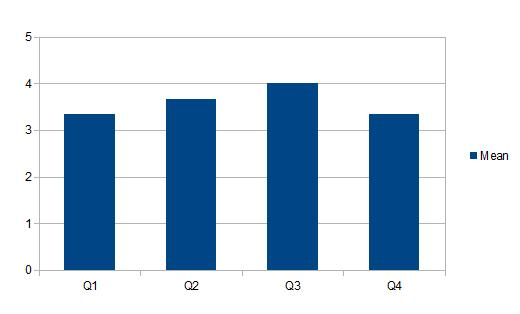
\includegraphics[scale=0.60]{inferinformation.jpg}
\end{subfigure}
\begin{subfigure}{\textwidth}
  \begin{description}
	\item[Q1]I could infer the underlying data distribution of a dataset/datasets 
	\item[Q2]While interacting with the tag cloud, I could identify outliers of a dataset/datasets
	\item[Q3]In a dataset/datasets, I could distinguish which tags had similar (data) characteristics
	\item[Q4]I could distinguish a relationship between one data variable and another data variable
  \end{description}
\end{subfigure}
\caption{\textit{Are users able to infer general information about the data from interacting with the visualisation? What kind of information?}}
\label{fig:inferinformation}
\end{figure}

\paragraph{Are users able to infer general information about the data from interacting with the visualisation? What kind of information? (Figure~\vref{fig:inferinformation})}

All users were able to infer the underlying data distribution (ranging from one dataset to all datasets), although with various levels of difficulty. All users were able to identifier outliers in a dataset and distinguish tags which had similar data characteristics. One evaluator commented they “found it difficult to choose the right mappings ” when trying to distinguish relationships between data variables.

\begin{figure}[!htb]
\centering
\begin{subfigure}{.5\textwidth}
	\centering
	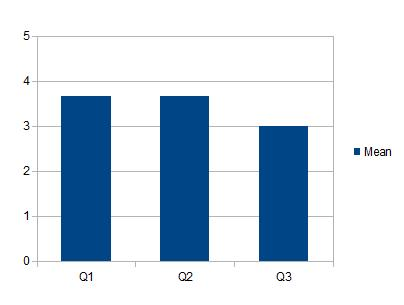
\includegraphics[scale=0.50]{backgroundcolour.jpg}
\end{subfigure}%
\begin{subfigure}{.5\textwidth}
  \begin{description}
	\item[Q1]Tag clouds were easier to read with background colour around the text
	\item[Q2]Background colour around the text enhanced my knowledge of a particular dataset/s
	\item[Q3]I forgot that I could put the colour around the background of the tag 
  \end{description}
\end{subfigure}
\caption{\textit{Does background colour around the text make data easier to understand?}}
\label{fig:backgroundcolour}
\end{figure}

\paragraph{Does background colour around the text make data easier to understand? (Figure~\vref{fig:backgroundcolour})}

Background colour was used minimally and evaluators required prompting about the option of putting background colour around the text. Although once used, most agreed it made the tag cloud easier to read.

\paragraph{Is a spiral or typewriter layout preferred? For what kinds of information?}

Evaluators did not establish a clear preference for spiral or typewriter layout for any particular dataset. The comment was made that ``it really depended on the variables mapped''. One user felt that the spiral layout was useful for finding data with similar characteristics and that the typewriter layout affected user perception unnaturally, with arbitrary points for line breaking creating a disjoint in the data. However typewriter layout was perceived as useful for textual labels that benefited from being displayed in alphabetical order. There was an expectation by one evaluator that data with similar characteristics might cluster together or make exact circles in rows around the centre when using the spiral layout.

\begin{figure}[!htb]
\centering
\begin{subfigure}{.5\textwidth}
	\centering
	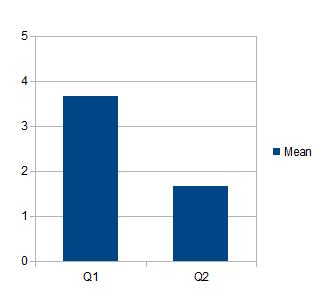
\includegraphics[scale=0.50]{datamapping.jpg}
\end{subfigure}%
\begin{subfigure}{.5\textwidth}
  \begin{description}
	\item[Q1]I found it useful to map a data variable to more than one tag cloud visual feature
	\item[Q2]I didn't try to map a data variable to more than one tag cloud visual feature
  \end{description}
\end{subfigure}
\caption{\textit{Is it useful to map a single data variable to multiple visual features?}}
\label{fig:datamapping}
\end{figure}

\paragraph{Is it useful to map a single data variable to multiple visual features? (Figure~\vref{fig:datamapping})}

All the users tried mapping a single data variable to multiple visual features. Users agreed it was useful to map a single data variable to multiple visual features. When mapping multiple data variables to multiple visual features the comment was made that the tag cloud ``became less useful when mapping more than two data variables''.


% ------------------------------------------------------------------------

%%% Local Variables: 
%%% mode: latex
%%% TeX-master: "../thesis"
%%% End: 
